\section{Data Preparation}
The data analysis performed in the previous section revealed some flaws in the dataset. The two most noticeables are the presence of outliers and the population imbalance between the two classes. These two flaws are known for harming the learning of most ML models. Differents attemps at solving these issues are presented in this section.

\subsection{Outliers}

\subsection{Balance Classes}
\label{balance_classes}
The following paragraphs deal with class balancing, explaining the importance of balanced classes and three different approaches two rectify the imbalance.\\

As said in the previous section, a mere 0.008\% of the population is defective individuals. In other words, the class of individuals which needs to be detected is truly under-represented in the dataset.
Without any pre-processing such a dataset is very unlikely to give good results with most of the ML models. As shown in Figure \ref{data_preparation_1}, there are not enough defective individuals for the classfifier to properly learn how to distinguish a defective individual from a valid individual. As a result, the classifier simply over-fit the valid class.\\

\noindent
\begin{minipage}[!hc]{0.12\textwidth}
   \textbf{Remarque}
\end{minipage}
\vrule\enskip\vrule\quad\begin{minipage}{\dimexpr 0.87\textwidth-0.8pt-1.5em}
Over-fitting the over-represented class is very hazardous as the accuracy of the classifier will remain really high eventhough the classifier is not classifying anything. Hopefully the confusion matrix shows the classification details.
\end{minipage}\\

\begin{figure}
    \center
    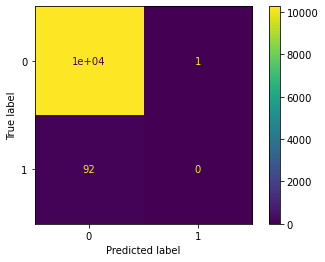
\includegraphics[scale=.5]{img/data_preparation_1.png}
    \caption{Confusion matrix of a k-Nearest Neighbors classifier with the base dataset}
    \label{data_preparation_1}
\end{figure}

The easiest method to deal with unbalanced classes is to remove valid individuals from the training dataset. This process is fairly straight forward (valid individuals can be randomly selected in the dataset) and does not require a lot of processing (selected individuals are simply removed).\\
Figure \ref{data_preparation_2} clearly shows that the classifier is not over-fitting the valid class anymore. In that sense, the results are better but they are still far from what is expected from a performant classifier.\\
This method is very arguable for two reasons.\\
Deleting individuals obviously implies a loss of data. Eventhough the individuals are randomly selected, some important features can disappear. In other words, the remaining data is not necessarily representative of the global population.\\
On top of that, the resulting dataset is smaller meaning the model will have less instances to learn on. In this problem, this will dramatically impact the results because there is already few data.\\

\begin{figure}
    \center
    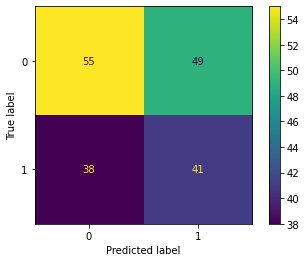
\includegraphics[scale=.5]{img/data_preparation_2.png}
    \caption{Confusion matrix of a k-Nearest Neighbors classifier with the dataset balanced by removing individuals}
    \label{data_preparation_2}
\end{figure}

Of course it is also possible to work the other way around and artificially create individuals instead of deleting others. The easiest method is actually to duplicate defective items until there are as many as the valid ones. This compensate the imbalance between the two classes without knowing anything about the features values. Figure \ref{data_preparation_3} shows the effect on the classifier is significant.\\
Another way that has been implemented during this project is to slightly modify individuals during the duplication. This way new individuals are actually new individuals (not only duplicates) adding information to the overall dataset. This method assumes individuals from the same class are close to one another on every dimension (i.e. regarding every feature) and changing a feature's value by a small amount will not induce a change of class. The way it has been implemented is surely not ideal but rather intuitive. A random amount of features are selected during each "duplication" and the value is modified by a very small percentage (typically 0.005).\\

\begin{figure}
    \center
    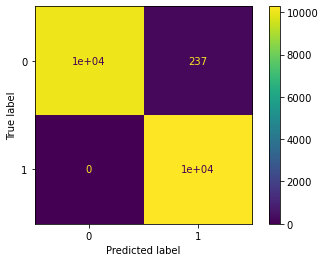
\includegraphics[scale=.5]{img/data_preparation_3.png}
    \caption{Confusion matrix of a k-Nearest Neighbors classifier with the dataset balanced by duplicating individuals}
    \label{data_preparation_3}
\end{figure}

The final method in order to balance classes consists in leaving the classes inbalanced in the dataset but during computation attributing a more significant weight to the individuals from the under-represented class. Technically speaking this is equivalent to duplicating individuals but it requires less memory, it is easier for computation and is already implemented for some algorithms from well known ML libraries.  